%
%\pdfinfo { /Title  (PhD Dessertation)
%               /Creator (TeX)
%               /Producer (pdfTeX)
%               /Author (AmritaWNA)
%               /CreationDate (D:20220629)  %format D:YYYYMMDD
%               /ModDate (D:20220629)
%               /Subject (Writing a Dessertation in LaTeX)
%               /Keywords (PhD, Qualifying ReportThesis)}
%    \pdfcatalog { /PageMode (/UseOutlines)
%                  /OpenAction (fitbh)  }

%input macros (i.e. write your own macros file called MacroFile1.tex)
%\include{Macros/MacroFile1}

\documentclass[oneside,times, 11pt,numbered,onehalfspacing]{CUEDthesisPSnPDF}
% \documentclass[
% 11pt, % The default document font size, options: 10pt, 11pt, 12pt
% %oneside, % Two side (alternating margins) for binding by default, uncomment to switch to one side
% english, % ngerman for German
% singlespacing, % Single line spacing, alternatives: onehalfspacing or doublespacing
% %draft, % Uncomment to enable draft mode (no pictures, no links, overfull hboxes indicated)
% %nolistspacing, % If the document is onehalfspacing or doublespacing, uncomment this to set spacing in lists to single
% %liststotoc, % Uncomment to add the list of figures/tables/etc to the table of contents
% %toctotoc, % Uncomment to add the main table of contents to the table of contents
% %parskip, % Uncomment to add space between paragraphs
% %nohyperref, % Uncomment to not load the hyperref package
% headsepline, % Uncomment to get a line under the header
% %chapterinoneline, % Uncomment to place the chapter title next to the number on one line
% %consistentlayout, % Uncomment to change the layout of the declaration, abstract and acknowledgements pages to match the default layout
% ]{CUEDthesisPSnPDF} % The class file specifying the document structure

%    
% Change the Title as per your details
\title{Thesis Title} 
%"PhD Qualifying Exam Report submitted in partial fulfillment of the degree "-go to File -> CUEDthesisPSnPDF.cls and change here \newcommand{\submittedtext}{{PhD Qualifying Exam Report submitted in partial fulfillment of the degree of}}
\degree{Doctor of Philosophy \\[1ex]in \\[1ex]WIRELESS NETWORKS AND APPLICATIONS}%Change as Major Dissertation/Minor Dissertation
% The year and Month the degree will be officially conferred
\degreedate{\today}      
% Change the Author name to full name of the person submitting the report.              
\author{Name \\ AM.EN.D*WNA1X1XX}
% Change the Guide name to full name of the Guide.  
\guide{Dr. Thesis Advisor Name}
% Change the register no.  
\regno{AM.EN.D*WNA1X1XX}
% Change the Academic Year
\academicyear{2022-23}
\vspace{25pt}
\crest{
\includegraphics[scale=1]{figs/amrita-logo.png}}
\vspace{30pt}
\collegeordept{\small{CENTER FOR WIRELESS NETWORKS AND APPLICATIONS}}
\university{AMRITA VISHWA VIDYAPEETHAM ,\\[1ex] (Estd. U/S 3 of the UGC Act 1956) Amritapuri  Campus \\[1ex] Kollam - 690525}
\crestsmall{
\includegraphics[scale=1]{figs/amrita-logo.png}}
\frontmatter 
\begin{document}
\maketitle
\pagenumbering{roman}
%USE FOR DISSERTATION REPORTS ONLY or IF NEEDED
\begin{center}
{\normalsize {\bfseries{ CENTER FOR WIRELESS NETWORKS AND APPLICATIONS	\\[1ex]}}}
{\normalsize {\bfseries{AMRITA VISHWA VIDYAPEETHAM ,\\[1ex] (Estd. U/S 3 of the UGC Act 1956) Amritapuri  Campus \\[1ex] Kollam -690525\\[1ex]}}}
	
\includegraphics[scale=1]{figs/amrita-logo.png}
	\rmfamily\bfseries\upshape\Large
	
	
BONAFIDE CERTIFICATE \\[2ex] % Insert your Project title here
\end{center}
		%\vspace{1pt}	
%\rmfamily\mdseries\upshape\normalsize
%change bonafide details as per your department credentials					
\hspace{1.2 cm}This  is  to  certify  that  the Qualifying Exam Report  entitled  \textbf{''Thesis Title''} submitted by Ms/Mr. Student Name (AM.EN.P2WNA*****), in partial fulfillment of the requirements for the award of Degree of Master of Technology in Wireless Networks and Applications from Amrita Vishwa Vidyapeetham, is a bonafide record of the work carried out by her under my guidance and supervision at Amrita School of Engineering, Amritapuri during Semester 4 of the academic year 2022-2023
\vspace{30pt}
\begin{flushleft}
Dr. Thesis Advisor \hspace{140pt} Dr. HoD Name\\
\vspace{3pt}
Thesis Adviser \hspace{190pt} Head of the Department\\
\vspace{30pt}
Dr Thesis Co-Adviser Name\hspace{140pt}\\
\vspace{3pt}
Thesis Co-Adviser\\
\vspace{35pt} 
Examiner 1   \hspace{209pt} Examiner 2 \\              
\end{flushleft}

% \begin{flushleft}
% \vspace{5pt}
% Place	:	Amritapuri \\
% Date	:	July 24, 2020
% \end{flushleft}

\pagebreak
%%DHANESH RAJ
\begin{center}
  {\normalsize {\bfseries{AMRITA CENTER FOR WIRELESS NETWORKS AND APPLICATIONS	\\[1ex]}}}

    {\normalsize {\bfseries{AMRITA VISHWA VIDYAPEETHAM ,\\[1ex] (Estd. U/S 3 of the UGC Act 1956) Amritapuri  Campus \\[1ex] Kollam -690525\\[1ex]}}}
    
\includegraphics[scale=1]{figs/amrita-logo.png}\\[1ex]
		
    \rmfamily\bfseries\upshape\Large
				DECLARATION \\[2ex]
    %\includegraphics[width=30mm]{UniEmblem}
    
    \end{center}
	\vspace{2pt}
I, \textbf{Mr. Student Name, Reg No: AM.EN.D*WNAxxxxx}, hereby declare that this project entitled \textbf{``Thesis Title``} is a record of the original work done by me under the guidance of \textbf{Dr. Thesis Name}, Center for Wireless Networks And Applications, Amrita Vishwa Vidyapeetham, that this work has not formed the basis for any degree/diploma/associationship/fellowship or similar awards to any candidate in any university to the best of my knowledge.

\vspace{60pt}
\begin{flushleft}
Place	:	Amritapuri\\[1ex]% PRint the place and date

Date	:	\date{\today} \\[15ex]

Signature of the Student \hspace{116pt}	Signature of the Thesis Adviser
\end{flushleft}

%set the number of sectioning levels that get number and appear in the contents
\setcounter{secnumdepth}{3}
\setcounter{tocdepth}{3}


\setlength{\parindent}{0pt} %Full block style
\setlength{\parskip}{11pt} %Assumes 11pt type
\hfuzz2pt % Don't bother to report over-full boxes if over-edge is < 2pt
%%Prefatory material
% Thesis Dedictation ---------------------------------------------------

\begin{dedication} %this creates the heading for the dedication page
\begin{figure}[t] %inserts the figure at the top of the page t denotes the top of the page %[!htbp]
  \begin{center}
    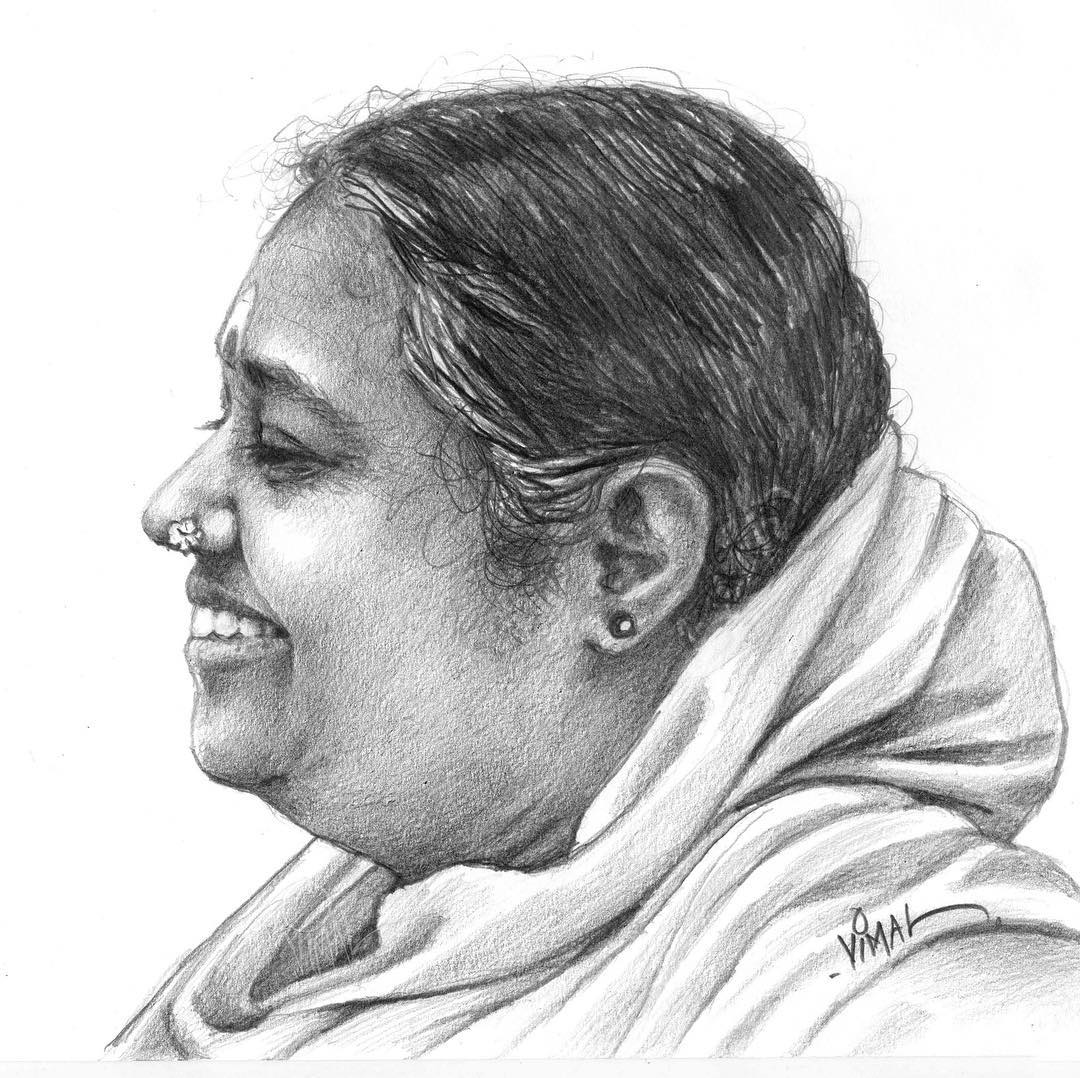
\includegraphics[scale=0.24]{figs/amma.png}
  \end{center}
\end{figure} 
I would like to dedicate this thesis to AMMA, Sri Mata Amritanandamayi Devi and my loving parents.

''Any transformation brought upon society by education devoid of values is superficial '' - Amma

\end{dedication}

% ----------------------------------------------------------------------

%%% Local Variables: 
%%% mode: latex
%%% TeX-master: "../thesis"
%%% End: 

\cleardoublepage
% Jury ====================================================================

\pdfbookmark[1]{Doctoral Committee Members}{Doctoral Committee Members}
\chapter*{Doctoral Committee Members}

\noindent \textsc{Dr. Name 1}, University Name 1 (Advisor) 

\noindent \textsc{Dr. Name 2}, University Name 2 (Co-Advisor) 

\noindent \textsc{Dr. Name 3}, University Name 3  

\noindent \textsc{Dr. Name 4}, University Name 4  

\noindent \textsc{Dr. Name 5}, University Name 5  

\noindent \textsc{Dr. Name 6}, University Name 6 (Coordinator)  %comment if not necessary
% Thesis Abstract -----------------------------------------------------
%\begin{abstractslong}    %uncommenting this line, gives a different abstract heading
\begin{abstracts}   
\addcontentsline{toc}{chapter}{Abstract} % adds an entry to the table of contents

\lipsum[3-5]

\end{abstracts}
%\end{abstractlongs}


% ----------------------------------------------------------------------


%%% Local Variables: 
%%% mode: latex
%%% TeX-master: "../thesis"
%%% End: 
% \setlength{\parskip}{0pt} %Assumes 11pt type
\tableofcontents
\newpage
\listoffigures
\newpage
\listoftables
\mainmatter
\pagenumbering{arabic}
%%% Thesis Introduction --------------------------------------------------
\chapter{Introduction}\label{chapter:intro}
\setlength{\parindent}{4em}
\setlength{\parskip}{1em}
\markboth{}{\MakeUppercase{Title Case}}
\section{Research Motivation and Challenges}
\lipsum[3-4]
\section{Problem Definition}
\begin{itemize}
\item \cite{Ref1}
\item \cite{Ref2}
\end{itemize}
% \begin{figure}[!h]
% \centering
% \includegraphics[scale=0.5]{figname.jpeg}
% \caption{Picture Title}
% \label{fig:label1}
% \end{figure}

%%%%%%%%%%%%%%%%%%%%%%%%%%%%%%%%%%%%%%%%%%%%%%%%%%%%%%
\section{Objectives}
The basis for the overall framework is developed by:

\begin{itemize}
    \item 
    \item 
    \item 
\end{itemize}
%%%%%%%%%%%%%%%%%%%%%%%%%%%%%%%%%%%%%%%%%%%%%%%%%%%%%%
\section{Thesis Outline}
The thesis is outlined as follows
\begin{itemize}
\item 
\end{itemize}

%%%COPY SAME FILE TO CREATE THE REPORT

%%%COPY SAME FILE TO CREATE THE REPORT








%%% Thesis Introduction --------------------------------------------------
\chapter{Related Work}\label{chapter:relatedwork}
\setlength{\parindent}{4em}
\setlength{\parskip}{1em}
\markboth{}{\MakeUppercase{Title Case}}
\section{Related Work}
\lipsum[3-4]
\section{Problem Definition}
\begin{itemize}
\item \cite{Ref1}
\item \cite{Ref2}
\end{itemize}
\subsection{Latex Tables}
\href{Online Table}{https://www.tablesgenerator.com/}
%%to generate quick tables use www.latextablegenerator.com
%%tospan across full page \begin{table*}[h!] --- \end{table*}
%%subfig and subcaption option if needed refer
\begin{table}[h!]
  \begin{center}
    \caption{More columns.}
    \label{tab:table1}
    \begin{tabular}{l|l|r|l}
      \textbf{Value 1} & \textbf{Value 2} & \textbf{Value 3} & \textbf{Value 4}\\ % <-- added & and content for each column
      $\alpha$ & $\beta$ & $\gamma$ & $\delta$ \\ % <--
      \hline
      1 & 1110.1 & a & e\\ % <--
      2 & 10.1 & b & f\\ % <--
      3 & 23.113231 & c & g\\ % <--
    \end{tabular}
  \end{center}
\end{table}
\section{Figures in Latex}
% https://latex-tutorial.com/subfigure-latex/
%%PACKAGES NEEDED - \usepackage{graphicx}
\begin{figure}[!h]%htbp as options
\begin{center}
  
\includegraphics[scale=0.6]{figs/research.png} %use textwidth/linewidth for more option
  \caption{Research}
  \label{fig:Research}
\end{center}
\end{figure}
This is my \ref{fig:Research} here
\begin{figure}[h!]%%%htbp 
\centering
\subfigure[Caption 1]{
    
\includegraphics[width=5.5cm]{figs/research.png}
    }
\quad
\subfigure[Caption 2]{
    
\includegraphics[width=5.5cm]{figs/research1.png}
}
\quad
\subfigure[Caption 3]{
    
\includegraphics[width=5.5cm]{figs/research.png}
\label{fig:label13}} % difference in this line
\caption{examples}\label{fig:label1} 
\end{figure}
This is my \ref{fig:label1} here
%%%COPY SAME FILE TO CREATE THE REPORT
\subsection{Equation in Latex}
\href{online latex equation}{https://latex.codecogs.com/eqneditor/editor.php}
%visit https://latex.codecogs.com/eqneditor/editor.php to generate online eqiuuations
\begin{equation}
  1 + 2 = 3 
\end{equation}%%use * for removing equation number
\begin{equation*}
  1 = 3 - 2
\end{equation*}
\begin{align*}
  1 + 2 &= 3\\
  1 &= 3 - 2
\end{align*}






%%% Thesis Introduction --------------------------------------------------
\chapter{Publications}\label{chapter:publication}
% \ifpdf
%     \graphicspath{{Introduction/IntroductionFigs/PNG/}{Introduction/IntroductionFigs/PDF/}{Introduction/IntroductionFigs/}}
% \else
%   \graphicspath{{Introduction/IntroductionFigs/EPS/}{Introduction/IntroductionFigs/}}
% \fi
\setlength{\parindent}{4em}
\setlength{\parskip}{1em}
\markboth{}{\MakeUppercase{Title Case}}
\section{Journal}
\begin{itemize}
    \item 
    \item 
\end{itemize}
\section{Conferences}
\begin{itemize}
    \item \cite{Ref1} S. L. S, D. Raj and S. Ponnekanti, "Connectivity Platform to Deliver Sync as a Service for 5G Digital Enterprise," 2019 International Conference on Wireless Communications Signal Processing and Networking (WiSPNET), 2019, pp. 530-533, doi: 10.1109/WiSPNET45539.2019.9032866.
    \item \cite{Ref2} P. Gopalakrishnan et al., "Routing protocol Analysis for Heterogeneous Nodes in a Dynamic and Sparse Environment," 2020 11th International Conference on Computing, Communication and Networking Technologies (ICCCNT), 2020, pp. 1-7, doi: 10.1109/ICCCNT49239.2020.9225354.
\end{itemize}
\clearpage
\begin{spacing}{0.9}
\addcontentsline{toc}{chapter}{\protect\numberline{}{Bibliography}}
% \includepdf[pages={1-4}]{final} %%Paper Submitted Pages
\bibliographystyle{ieeetr}
\cleardoublepage
\renewcommand{\bibname}{References}% changes default name Bibliography to References 
\bibliography{references}%
\backmatter % book mode only
\end{spacing}

\begin{appendices} % Using appendices environment for more functunality

%!TEX root = ../thesis.tex
% ******************************* Thesis Appendix A ****************************
\chapter{Program Code Python} 

\section*{Code for Wireless Network Simulation}

\subsection*{Code for Propagation Loss}
\begin{verbatim}
import heapq

def calculate_distances(graph, starting_vertex):
    distances = {vertex: float('infinity') for vertex in graph}
    distances[starting_vertex] = 0

    pq = [(0, starting_vertex)]
    while len(pq) > 0:
        current_distance, current_vertex = heapq.heappop(pq)

        # Nodes can get added to the priority queue multiple times. We only
        # process a vertex the first time we remove it from the priority queue.
        if current_distance > distances[current_vertex]:
            continue

        for neighbor, weight in graph[current_vertex].items():
            distance = current_distance + weight

            # Only consider this new path if it's better than any path we've
            # already found.
            if distance < distances[neighbor]:
                distances[neighbor] = distance
                heapq.heappush(pq, (distance, neighbor))

    return distances


example_graph = {
    'U': {'V': 2, 'W': 5, 'X': 1},
    'V': {'U': 2, 'X': 2, 'W': 3},
    'W': {'V': 3, 'U': 5, 'X': 3, 'Y': 1, 'Z': 5},
    'X': {'U': 1, 'V': 2, 'W': 3, 'Y': 1},
    'Y': {'X': 1, 'W': 1, 'Z': 1},
    'Z': {'W': 5, 'Y': 1},
}
print(calculate_distances(example_graph, 'X'))

\end{verbatim}
\chapter{Program Code Python} 
\section{calculating path loss in a point-to-point analysis}
\begin{verbatim}
    

import dataclasses
from decimal import Decimal
from pathlib import Path
import os
import subprocess
import re
import tempfile
from typing import Union, NamedTuple, Tuple
from typing_extensions import Literal


PolarizationType = Union[Literal[0], Literal[1]]
RadioClimateType = Union[
    Literal[1],
    Literal[2],
    Literal[3],
    Literal[4],
    Literal[5],
    Literal[6],
    Literal[7],
    Literal[8],
    Literal[9],
]
FreeSpacePathLossDecibels = Decimal
IWOTMPathLossDecibels = Decimal
FieldStrengthDBuV = Decimal


class SplatReportException(Exception):
    def __init__(self, *args, **kw):
        self.report_text = kw.pop("report_text", None)
        super().__init__(*args, **kw)


class LRPFields(NamedTuple):
    erp_W: Decimal
    frequency_MHz: Decimal
    polarization: PolarizationType
    radio_climate: RadioClimateType
    earth_dielectric_constant: Decimal = Decimal("15.000")
    earth_conductivity: Decimal = Decimal("0.005")
    atmospheric_bending_constant: Decimal = Decimal("301.000")
    fraction_situations: Decimal = Decimal("0.50")
    fraction_time: Decimal = Decimal("0.50")


class QTHFields(NamedTuple):
    name: str
    latitude: Decimal
    longitude_EtoW: Decimal
    height_m: Decimal


@dataclasses.dataclass
class Transmitter:
    name: str
    latitude: Decimal
    longitude_WtoE: Decimal
    height_m: Decimal
    eirp_W: Decimal
    frequency_MHz: Decimal
    polarization: PolarizationType
    # Could be moved to a `Fresnel` class that specifies data about the environment:
    radio_climate: RadioClimateType

    def __post_init__(self):
        def _convert_to_decimal(val):
            if isinstance(val, Decimal):
                return val
            if isinstance(val, float):
                return Decimal(str(val))
            return Decimal(val)

        for field in dataclasses.fields(self):
            if field.type is Decimal:
                setattr(
                    self, field.name, _convert_to_decimal(getattr(self, field.name))
                )

    def to_qthfields(self) -> QTHFields:
        return QTHFields(
            name=self.name,
            latitude=self.latitude,
            longitude_EtoW=(Decimal("360") - self.longitude_WtoE) % 360,
            height_m=self.height_m,
        )

    def to_lrpfields(self) -> LRPFields:
        return LRPFields(
            erp_W=self.eirp_W / Decimal("1.64"),
            frequency_MHz=self.frequency_MHz,
            polarization=self.polarization,
            radio_climate=self.radio_climate,
        )


@dataclasses.dataclass
class Receiver:
    name: str
    latitude: Decimal
    longitude_WtoE: Decimal
    height_m: Decimal

    def __post_init__(self):
        def _convert_to_decimal(val):
            if isinstance(val, Decimal):
                return val
            if isinstance(val, float):
                return Decimal(str(val))
            return Decimal(val)

        for field in dataclasses.fields(self):
            if field.type is Decimal:
                setattr(
                    self, field.name, _convert_to_decimal(getattr(self, field.name))
                )

    def to_qthfields(self) -> QTHFields:
        return QTHFields(
            name=self.name,
            latitude=self.latitude,
            longitude_EtoW=(Decimal("360") - self.longitude_WtoE) % 360,
            height_m=self.height_m,
        )


QTH_TEMPLATE = "\n".join(
    ["{name}", "{latitude}", "{longitude_EtoW}", "{height_m} meters"]
)

LRP_TEMPLATE = "\n".join(
    [
        "{earth_dielectric_constant}	; Earth Dielectric Constant (Relative"
        " permittivity)",
        "{earth_conductivity}; Earth Conductivity (Siemens per meter)",
        "{atmospheric_bending_constant}	; Atmospheric Bending Constant (N-Units)",
        "{frequency_MHz}	; Frequency in MHz (20 MHz to 20 GHz)",
        "{radio_climate}	; Radio Climate",
        "{polarization}	; Polarization (0 = Horizontal, 1 = Vertical)",
        "{fraction_situations}	; Fraction of Situations",
        "{fraction_time}	; Fraction of Time",
        "{erp_W} ; ERP",
    ]
)

REPORT_FILENAME_TEMPLATE = "{transmitter.name}-to-{receiver.name}.txt"


def splat_report_values(
    terrain_folder: str,
    cities_filepath: str,
    transmitter: Transmitter,
    receiver: Receiver,
    timeout=2,
) -> Tuple[FreeSpacePathLossDecibels, IWOTMPathLossDecibels, FieldStrengthDBuV]:
    """
    :raise: TimeoutExpired in case the subprocess takes too long
    :raise: SplatReportException in case the Splat report doesn't look as expected
    """
    with tempfile.TemporaryDirectory() as tmpdirname:
        tmpdir_path = Path(tmpdirname)
        transmitter_qth_path = tmpdir_path / f"transmitter-{transmitter.name}.qth"
        transmitter_lrp_path = tmpdir_path / f"transmitter-{transmitter.name}.lrp"
        receiver_qth_path = tmpdir_path / f"receiver-{receiver.name}.qth"

        with transmitter_qth_path.open(
            "w"
        ) as transmitter_qth_file, transmitter_lrp_path.open(
            "w"
        ) as transmitter_lrp_file, receiver_qth_path.open(
            "w"
        ) as receiver_qth_file:
            transmitter_qth_file.write(
                QTH_TEMPLATE.format(**transmitter.to_qthfields()._asdict())
            )
            transmitter_lrp_file.write(
                LRP_TEMPLATE.format(**transmitter.to_lrpfields()._asdict())
            )
            receiver_qth_file.write(
                QTH_TEMPLATE.format(**receiver.to_qthfields()._asdict())
            )

        args = [
            "splat",
            "-metric",
            "-s",
            f"{cities_filepath}",
            "-d",
            f"{terrain_folder}",
            "-t",
            str(transmitter_qth_path),
            "-r",
            str(receiver_qth_path),
        ]
        subprocess.run(
            args,
            cwd=str(tmpdir_path),
            stdout=subprocess.PIPE,
            stderr=subprocess.PIPE,
            universal_newlines=True,
            check=True,
            timeout=timeout,
        )

        output_path = tmpdir_path / REPORT_FILENAME_TEMPLATE.format(
            transmitter=transmitter, receiver=receiver
        )
        # Encoding copied from Splat gnuplot files:
        with open(str(output_path), encoding="iso_8859_1") as report_file:
            report_text = report_file.read()
            matches = re.search(
                r"Free space path loss: (\d*\.\d*) dB"
                r".*?"
                r"ITWOM Version 3.0 path loss: (\d*\.\d*) dB"
                r".*?"
                r"(\d*\.\d*) dBuV/meter",
                report_text,
                flags=re.DOTALL,
            )
            if matches:
                return (
                    Decimal(matches.group(1)),
                    Decimal(matches.group(2)),
                    Decimal(matches.group(3)),
                )

        raise SplatReportException(
            "Error reading splat report", report_text=report_text
        )


def test1():
    terrain_folder = os.environ["TERRAIN_FOLDER"]
    cities_filepath = os.environ["CITIES_FILEPATH"]
    transmitter = Transmitter(
        name="Menesble",
        latitude=Decimal("47.78194"),
        longitude_WtoE=Decimal("4.90917"),
        height_m=Decimal("41.0"),
        eirp_W=Decimal("80.0"),
        frequency_MHz=Decimal("800.00"),
        polarization=1,
        radio_climate=5,
    )
    receiver = Receiver(
        name="Bure",
        latitude=Decimal("47.738787"),
        longitude_WtoE=Decimal("4.8892801"),
        height_m=Decimal("2.0"),
    )
    assert splat_report_values(
        terrain_folder, cities_filepath, transmitter, receiver
    ) == [Decimal("104.55"), Decimal("141.82"), Decimal("42.53")]


if __name__ == "__main__":
    test1()
\end{verbatim}

\end{appendices}




\end{document}
